\documentclass{beamer}
\usepackage{ulem}
\usepackage{tikz}
\usepackage{booktabs}
\usepackage{graphicx,threeparttable,caption}
\usetikzlibrary{shapes,snakes}
\usepackage[beamer,customcolors]{hf-tikz}
\usepackage{nicematrix}
\usepackage{xcolor}
\usepackage{makecell}
\usepackage{array}
\usepackage{csquotes}
\usepackage{csquotes}
\usepackage{minted}
\usepackage{animate}
\captionsetup{labelformat=empty,labelsep=none}

\graphicspath{ {./png/} }

\usetikzlibrary{
    arrows,
    arrows.meta,
    shapes,
    positioning,
    shadows,
    trees,
    calc
}

\tikzset{%
    >={Latex[width=2mm,length=2mm]},
    % Specifications for style of nodes:
    plain/.style = {},
    base/.style = {
        plain,
        rectangle, rounded corners, draw=black,
        minimum width=1cm, minimum height=1cm,
        text centered, font=\sffamily\tiny\bfseries,
        fill=white, align=center
    },
    app/.style = {base, ellipse},
    data/.style = {base, fill=gray!30},
    action/.style = {base, circle, fill=red!30},
    note/.style = {app, fill=yellow},
    hl/.style={
    set fill color=red!80!black!40,
    set border color=red!80!black
    }
}


\AtBeginSection[]{
  \begin{frame}
  \vfill
  \centering
  \begin{beamercolorbox}[sep=8pt,center,shadow=true,rounded=true]{title}
    \usebeamerfont{title}\insertsectionhead\par%
  \end{beamercolorbox}
  \vfill
  \end{frame}
}
\setbeamercolor{alerted text}{fg=red}
%\usecolortheme[orchid]{structure}
\usetheme[hideothersubsections]{PaloAlto}
\makeatletter
\patchcmd{\csq@bquote@i}{{#6}}{{\emph{#6}}}{}{}
\makeatother
%\usecolortheme{orchid}
%\usefonttheme{professionalfonts}
\newcommand{\soutthick}[1]{%
   \textcolor{red}{
   \renewcommand{\ULthickness}{1pt}%
      \sout{#1}%
   \renewcommand{\ULthickness}{.4pt}% Resetting to ulem default
   }
}
\newcommand{\centered}[1]{\begin{tabular}{l} #1 \end{tabular}}
\setbeamertemplate{section in toc}[square]
\setbeamertemplate{subsection in toc}[square]
\setbeamertemplate{section in sidebar}[shaded]
\setbeamertemplate{items}[square]
\setbeamercovered{transparent} 

\title[]{Introduction to Computational Social Science}
\subtitle{Working with the GDELT API}
\author[]{Mikołaj Biesaga\\ \small{\color{blue}{\href{mailto:m.biesaga@uw.edu.pl}{m.biesaga@uw.edu.pl}}}}
\institute{
\includegraphics[width = 4 cm]{uw.png}}
\date{April 29, 2025}
\begin{document}
\begin{frame}
   \titlepage
\end{frame}

\section[GDELT Project]{What is GDELT Project?}

\begin{frame}
   \frametitle{What is the GDELT Project?}
   \only<1>{
      \begin{definition}
         Global Database of Events, Language, and Tone (GDELT) project is a
         repository of global events and news articles. The GDELT Project monitors
         a \alert{sample} of the world's broadcast, print, and web news from nearly every
         corner of every country in over 100 languages and identifies the people,
         locations, organizations, themes, sources, emotions, counts, quotes,
         images and events driving our global society every second of every day,
         creating a free open platform for computing on the entire world.
      \end{definition}
   }
   \only<2>{
      \begin{itemize}
         \item It is updated every \alert{15 minutes}.
         \item Realtime translation of \alert{65 languages}.
         \item Three main data streams:
         \begin{enumerate}
            \item Physical activities (events) codified in 300 categories;
            \item Entities (people, organizations, places) and emotions;
            \item Visual narratives of the world's news imaginery.
         \end{enumerate}
         \item Sources, from hundreds of thousands of global media outlets to special collections like 215 years of digitized books, 21 billion words of academic literature spanning 70 years, human rights archives and even stream of almost 100 television stations across the US.
      \end{itemize}
   }
   \only<3>{
      \framesubtitle{CAMEO}
      \begin{itemize}
         \item CAMEO (Conflict and Mediation Event Observations) is a coding scheme for events.
         \item There is a list of 20 main categories of events, such as:
         \begin{enumerate}
            \item Make Public Statements;
            \item Appeal;
            \item Express Intent to Cooperate;
            \item ...
         \end{enumerate}
         \item Each event is coded with a CAMEO code, which consists of 3-4
         digits.
         \item For example, the CAMEO code 01 coresponds to Make Public Statements and 018 Make Emphatethic Comment.
      \end{itemize}
   }
   \only<4>{
      \framesubtitle{CAMEO}
      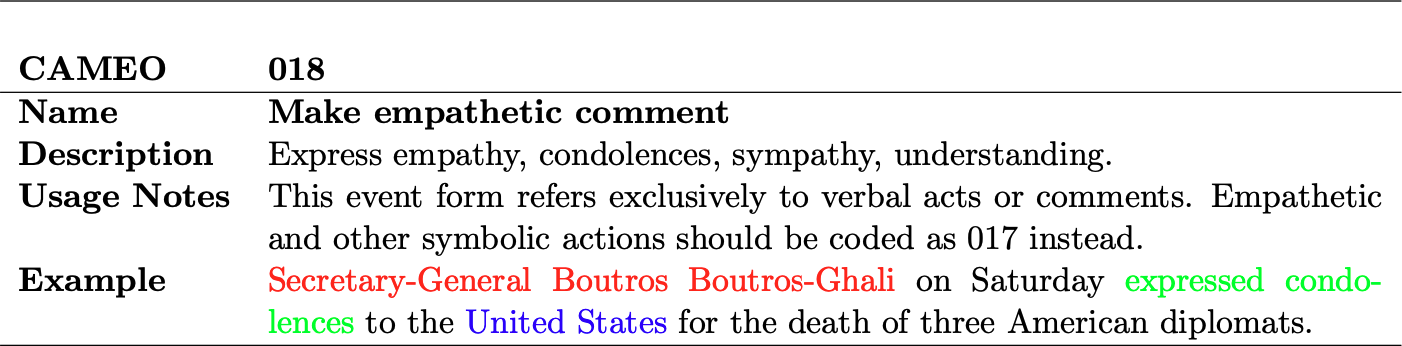
\includegraphics[width = \textwidth]{cameo.png}
   }
   \only<5>{
      \framesubtitle{Global Knowledge Graph}
      \begin{itemize}
         \item GKG is an array of highly sophisticated natural language
         processing algorithms (sic!) to each document to compute a range of
         codified metadata encoding key latent and contextual dimensions of the
         document.
         \item Among others these fields inform about:
         \begin{enumerate}
            \item Date;
            \item Source;
            \item Themes;
            \item Locations;
            \item Organizations;
            \item Persons;
            \item Tone.
         \end{enumerate}
      \end{itemize}
   }
\end{frame}

\section[Migration Studies]{Migration Studies}

\begin{frame}
   \frametitle{Societal response to Ukrainian refugee migration}
   \framesubtitle{Weisser, 2022}
   \begin{itemize}
      \item Eight weeks after the first shot was fired, the overall number of
      Ukrainians seeking protection abroad stood at 5.1 million (UNHCR, 2022a).
      \item Will non-government societal stakeholders, such as business or civil
      society representatives, maintain their levels of support for a prolonged
      period or can we expect levels of cooperation to fade quickly?
      \item Who becomes more likely to provide aid or express the intent to
      cooperate in the short run? Who disapproves or threatens?
      \item Whilst the influx of (large) refugee populations is typically
      associated with positive impulses for the local economy, attitudes towards
      refugees and political preferences of native residents edge towards a more
      hostile position. 
      \item Irrespective of the absence of adverse economic implications, public attitudes towards refugees can be volatile.
      Residents living near transit routes across the Balkan between 2010 and 2016 were much more sceptical about
      immigrants and their contribution to society (Ajzenman et al., 2022). Moreover, institutional trust and perceived
      political stability declined along these transit corridors. When it comes to supporting asylum seekers, European citi-
      zens display a distinct preference for those more likely to be easily integrated into labour markets or society, and
      those who are deemed more vulnerable (Bansak et al., 2016). Anti-refugee or anti-immigrant attitudes were found to
      be more prevalent amongst Europeans who are living in relative economic deprivation and who have fewer contact
      experiences with migrant groups (Albada et al., 2021). Similarly, prior contact in the form of friendships with minority
      group members translates into more positive attitudes towards newly arrived refugees (Lippard \& McNamee, 2021).
      \item Acceptance of individuals seeking protection due to war tends to be higher (Von Hermanni \& Neumann, 2019),
      yet can be lower for refugees from Eastern Europe, especially when fiscal concerns are factored in.
      \item Attitudes towards
      14682435, 2023, 4, Downloaded from https://onlinelibrary.wiley.com/doi/10.1111/imig.13071 by Pcp/University Of Warsaw, Wiley Online Library on [25/04/2025]. See the Terms and Conditions (https://onlinelibrary.wiley.com/terms-and-conditions) on Wiley Online Library for rules of use; OA articles are governed by the applicable Creative Commons License
      refugees may also be shaped by news media consumption (De Coninck, 2020): Frequent consumers of public broad-
      casters or quality newspapers are more likely to display positive attitudes towards refugees; the reverse applies to
      regular viewers of commercial broadcast networks. Frequent media coverage of migration issues may also increase
      immigration worries (Benesch et al., 2019).
      \item Overall, societal attitudes towards refugees depend strongly on the economic and institutional setting. Concom-
      itantly, changing attitudes have the potential to shape the politico-economic environment in host countries. This, in
      turn, implies that a timely evaluation of response dynamics is crucial to managing refugee migration and integration
      successfully.
   \end{itemize}

\end{frame}

\section[GDELT API]{GDELT API}
\begin{frame}
   \frametitle{API}
   \only<+>{
      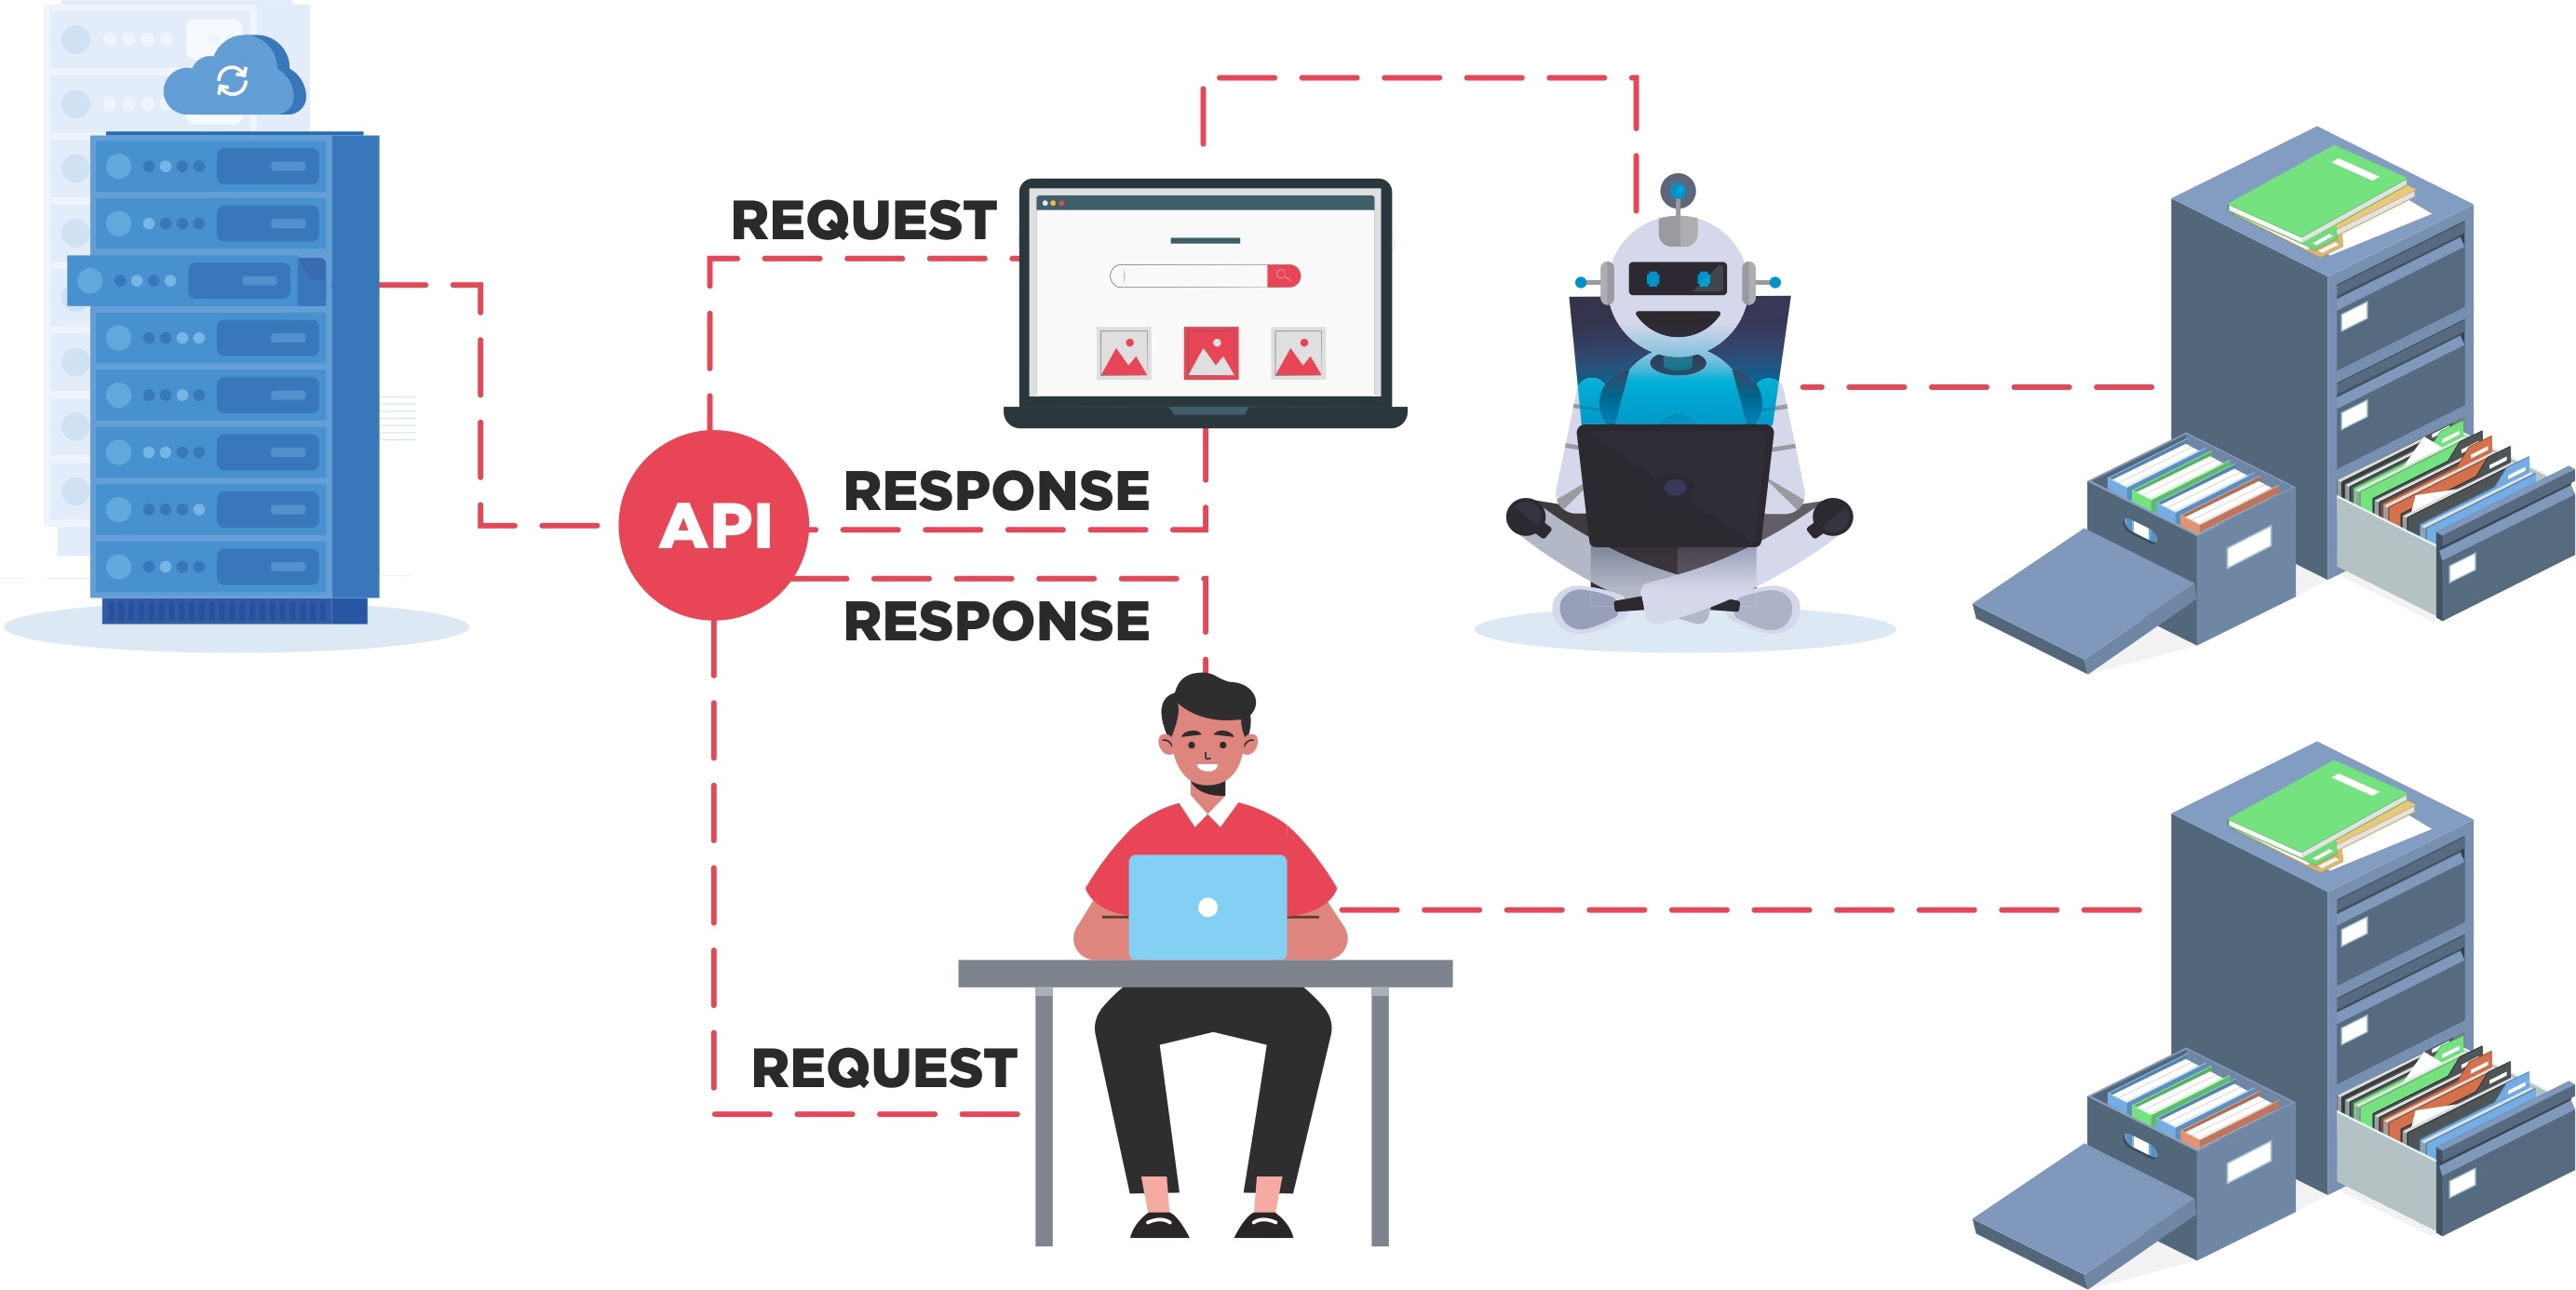
\includegraphics[width = \textwidth]{api.jpg}
   }
   \only<+>{
        \begin{definition}
            \emph{Aplication Programming Interface} is a communication protocol between a client and a server intended to simplify the building of client-side software. In other words, it is a contract between the client and the server which defines the format of possible requests and the format of the response (i.e. format of the data).
        \end{definition}
   }
   \only<+>{
      \framesubtitle{GDELT API}
      \begin{enumerate}
         \item Read the documentation
         \item Test the API in the web browser
         \item Extract the data using BigQuery
         \item Analyze the data
      \end{enumerate}
   }
\end{frame}


\end{document}